% !TEX root = 20230505_SHTSymposium.Presentation.tex

\title[MikroCT \& Histologie]{Was ist MikroCT und bringt das etwas Neues für die Histologie?}
\author{David Haberthür}
\date{5. Mai 2023 | Symposium Schweizerische Gesellschaft für Histologie-Technik}

\usetheme{UniBern}

%\includeonlyframes{current}
%then....
%\begin{frame}[label=current]
%\end{frame}

% Some often used abbreviations/commands
\newcommand{\everyframe}{100}% use only every nth frame for the animations
\newcommand{\imagewidth}{\linewidth}% set global image width
\newcommand{\imageheight}{0.618\paperheight}% set global image height
\newlength\imagewidth% needed for scalebars
\newlength\imagescale% needed for scalebars
\newcommand{\uct}{{\textmu}CT\xspace}% make our life easier

\usepackage[ngerman]{babel}
\usepackage[backend=biber,
	style=numeric,
	url=false,
	isbn=true,
	maxnames=1,
	sorting=none]{biblatex}
\addbibresource{../../Documents/library.bib}% FastSSD, Windows or Mac works (on Linux/FastSSD we generated a 'Document' folder at the correct level and `ln -s ~/P/Documents/library.bib .` to it)
\usepackage{standalone}
\usepackage{tikz}
	\usetikzlibrary{spy}
	\tikzset{shadowed/.style={preaction={transform canvas={shift={(1pt,-1pt)}},draw=ubRed}}}
\usepackage{shadowtext}% for the shadowed scalebar
	\shadowoffset{1pt}
	\shadowcolor{ubRed}
\usepackage{pgfplots}
	\pgfplotsset{compat=newest}
\usepackage[detect-all=true,
	range-phrase=--,
	range-units=single,
	per-mode=symbol,
	per-symbol=/]{siunitx}
\usepackage{microtype}
\usepackage[absolute,overlay]{textpos}%for the \source{} command
\usepackage[missing=main]{gitinfo2}% GitHub Actions don't pull in the commit hash, so we force the footer some lines down.
\usepackage{xspace}
\usepackage{ccicons}
\usepackage[version=4]{mhchem}
\usepackage{animate}
\usepackage{fontawesome5}
\usepackage{csquotes}
\usepackage{listings}
	\lstset{frame=single,
		%backgroundcolor = \color{lightgray},
		basicstyle=\tiny\ttfamily
		}
\usepackage{pgfplotstable}
\usepackage{booktabs}
\usepackage{colortbl}
\usepackage{multirow}
\usepackage{lipsum}%for alignment testing
\usepackage{mathastext}

% Define complementary colors to ubRed
\definecolor{ubRedComplementary1}{HTML}{00a1e6}
\definecolor{ubRedComplementary2}{HTML}{00e645}

% change tikz font to slide font
% https://tex.stackexchange.com/a/33329/828
\usepackage[eulergreek]{sansmath}
	\pgfplotsset{tick label style = {font=\sansmath\sffamily},
		every axis label = {font=\sansmath\sffamily},
		legend style = {font=\sansmath\sffamily},
		label style = {font=\sansmath\sffamily}
		}

% Globally thicker lines in with tikz
% https://tex.stackexchange.com/a/206769/828
\tikzset{every picture/.style={thick}}

% Acknowledge images just below them
% Based on https://tex.stackexchange.com/a/282637/828
\newcommand{\source}[2]{%
	% Print out (short) link under image, with small text
	\raisebox{-1.618ex}{%
		\makebox[0pt][r]{%
			\tiny\href{http://#1}{#1} #2%
			}%
		}%
	}%
\newcommand{\sourcecite}[2]{%
	% Cite (an image from) a reference
	\raisebox{-1.618ex}{%
		\makebox[0pt][r]{%
			\tiny From \cite{#1}, #2%
			}%
		}%
	}%
\newcommand{\sourcelink}[3]{%
	% Make the source command an \href{link}{text}
	\raisebox{-1.618ex}{%
		\makebox[0pt][r]{%
			\tiny\href{http://#1}{#2}, #3%
			}%
		}%
	}%

% Define us a custom footer *with* progress bar, based on https://tex.stackexchange.com/a/59749/828
\makeatletter
\def\progressbar@progressbar{}% the progress bar
\newcount\progressbar@tmpcounta% auxiliary counter
\newcount\progressbar@tmpcountb% auxiliary counter
\newdimen\progressbar@pbht%progressbar height
\newdimen\progressbar@pbwd%progressbar width
\newdimen\progressbar@rcircle% radius for the circle
\newdimen\progressbar@tmpdim% auxiliary dimension
\progressbar@pbwd=0.85\linewidth%
\progressbar@rcircle=1.5pt%
\def\progressbar@progressbar{%
	\progressbar@tmpcounta=\insertframenumber%
	\progressbar@tmpcountb=\inserttotalframenumber%
	\progressbar@tmpdim=\progressbar@pbwd%
	\multiply\progressbar@tmpdim by \progressbar@tmpcounta%
	\divide\progressbar@tmpdim by \progressbar@tmpcountb%
	\par%
		\mode<beamer>{%
			\begin{tikzpicture}%
				\draw[ubGrey] (0,0) -- ++ (\progressbar@pbwd,0);%
				\draw[draw=ubRed,fill=ubGrey] (\the\dimexpr\progressbar@tmpdim-\progressbar@rcircle\relax,.5\progressbar@pbht) circle (\progressbar@rcircle);%
			\end{tikzpicture}%
			\hfill%
			bit.ly/SHTuCT\xspace|\xspace v.\xspace\href{https://github.com/habi/Talk.2023.SHTSymposium/commit/\gitHash}{\gitAbbrevHash}\xspace|\xspace\insertframenumber/\inserttotalframenumber%
			}%
		\mode<handout>{%
			bit.ly/SHTuCT\hfill|\hfill%
			Handout: Version vom \today\hfill|\hfill%
			\insertframenumber/\inserttotalframenumber%
			}%
		\vspace{0.5ex}%
}
\addtobeamertemplate{footline}{}%
{%
	\begin{beamercolorbox}[wd=\paperwidth,center]{white}%
		\progressbar@progressbar%
	\end{beamercolorbox}%
}%
\makeatother

% Format bibliography for beamer
% http://tex.stackexchange.com/a/10686/828
\renewbibmacro{in:}{}
% http://tex.stackexchange.com/a/13076/828
\AtEveryBibitem{%
	\clearfield{journaltitle}
	\clearfield{pages}
	\clearfield{volume}
	\clearfield{number}
	\clearname{editor}
	\clearfield{issn}
	\clearfield{year}
}
% No parentheses around the (now empty) year: https://tex.stackexchange.com/a/147537/828
\renewcommand{\bibopenparen}{\addcomma\addspace}
\renewcommand{\bibcloseparen}{\addcomma\addspace}

% Redefine \footcite based on https://tex.stackexchange.com/a/453528/828
\DeclareCiteCommand{\footcite}[\mkbibfootnote]{%
	\usebibmacro{prenote}}{%
		\printnames[family-given]{labelname}%
		\newunit%
		\printfield{doi}%
		\newunit%
		\printlabeldateextra%
	}{\addsemicolon\space}{%
		\usebibmacro{postnote}%
	}%

% References as footnotes at the bottom of the slides
% https://tex.stackexchange.com/a/368760/828
\makeatletter
\renewcommand\@makefnmark{\xspace\hbox{\usebeamercolor[fg]{footnote mark}\usebeamerfont*{footnote mark}[\@thefnmark]}}
\renewcommand\@makefntext[1]{\tiny{\usebeamercolor[fg]{footnote mark}\usebeamerfont*{footnote mark}[\@thefnmark]}\enspace\usebeamerfont*{footnote} #1}
\makeatother

% Show current section at begin of sections, but only in presentation mode
\mode<beamer>{%
	\AtBeginSection[]{%
		\begin{frame}{Contents}
			\tableofcontents[currentsection,currentsubsection,hideothersubsections]
		\end{frame}
	}
}

% Slide transiton
%\addtobeamertemplate{background canvas}{\transfade[duration=0.5]}{}

% open in fullscreen
%\hypersetup{pdfpagemode=FullScreen}

% Move the text down a bit
% THIS IS A BIG HACK, IT SHOULD BE FIXED IN THE TEMPLATE
\addtobeamertemplate{frametitle}{}{\vspace*{0.75em}}

\begin{document}
% No footline on the title page
% http://tex.stackexchange.com/a/18829/828 helps us to achieve that
{%
	\setbeamertemplate{footline}{}%
	\begin{frame}%
		\maketitle
	\end{frame}%
}

%% Alignment frames to test the ugly text-block-movement hack above
%\begin{frame}[label=current]{Alignment frame}
%	\begin{tikzpicture}%
%		\def\cut{2}%
%		\draw [|-|,ultra thick] (0,\cut) -- (0,\textheight-\cut);%
%		\draw [<->,ultra thick] (0.5\textwidth,\cut) -- (0.5\textwidth,\textheight-\cut);%
%		\draw [|-|,ultra thick] (\textwidth,\cut) -- (\textwidth,\textheight-\cut);%
%	\end{tikzpicture}%
%\end{frame}
%
%\begin{frame}[allowframebreaks,label=current]{Alignment frame II}
%	\lipsum[1-3]
%\end{frame}

\begin{frame}
	\frametitle{Grüessech mitenang!}
	\begin{itemize}
		\item David Haberthür
		\begin{itemize}
			\item Physiker
			\item \href{https://boris.unibe.ch/2619/}{Doktorarbeit über höchstaufgelöste tomographische Bildgebung in der Lunge} am Institut für Anatomie der Universität Bern
			\item Post-Doc I: Tomographische Bildgebung von Allerlei an \href{https://www.psi.ch/sls/tomcat/}{TOMCAT} am \href{https://www.psi.ch/}{Paul Scherrer Institut}
			  und Mitarbeit am \href{http://globaldiagnostix.org}{GlobalDiagnostiX}-Projekt
			\item Post-Doc II \& Gegenwart: Tomographische Bildgebung von biomedizinischen Dingen in der \href{https://www.ana.unibe.ch/forschung/mikroct/research/}{\uct-Gruppe} am Institut für Anatomie der Universität Bern
		\end{itemize}
	\end{itemize}
\end{frame}

\begin{frame}
	\frametitle{\uct-Gruppe}
	\begin{columns}
		\begin{column}{0.61\linewidth}
			\begin{itemize}
				\item microangioCT~\cite{Hlushchuk2018}
				\begin{itemize}
					\item Angiogenese: Herz, Muskulatur~\cite{Nording2021} und Knochen
					\item Gefässe: (Mäuse) Gehirn~\cite{Hlushchuk2020}, (humane) Nerven~\cite{Wuthrich2020}, (human) Hautgewebe~\cite{Zubler2021} und Tumore
				\end{itemize}
				\item Muskulatur und Kiemen von Zebrafischen~\cite{MesserliAaldijk2020}
				\item Erkennung und Klassierung von Tumoren und Metastasen~\cite{Trappetti2021}
				\item Zusammenarbeit mit NMBE~\cite{Bochud2021} und Wissenschaftler:innen der Uni Bern~\cite{Halm2021,Haberthuer2023}
			\end{itemize}
		\end{column}
		\begin{column}{0.37\linewidth}
			\centering
			\includegraphics<1|handout:0>[width=\imagewidth]{./images/1172}%
			\only<1|handout:0>{\source{brukersupport.com}{}}
			\includegraphics<2>[width=\imagewidth]{./images/1272}%
			\only<2>{\source{bruker.com/skyscan1272}{}}
			\includegraphics<3|handout:0>[width=\imagewidth]{./images/2214}%
			\only<3|handout:0>{\source{bruker.com/skyscan2214}{}}
		\end{column}
	\end{columns}
\end{frame}

\begin{frame}{Inhalt}
	\tableofcontents
\end{frame}

\section{Bildgebung}
\begin{frame}
	\frametitle{Biomedizinische Bildgebung}%
	\begin{columns}%
		\begin{column}{0.37\linewidth}%
			\begin{itemize}%
				\item<1-|handout:1-> Biomedizinische Forschung%
				\item<1-|handout:1-> Zerstörungsfreie Bilder aus dem Inneren von verschiedensten Probenm%
				\item<2-|handout:1->(Kleine) Biomedizinische Probem%
			\end{itemize}%
		\end{column}%
		\begin{column}{0.61\linewidth}%
			\centering%
			\only<1-2|handout:1>{%
				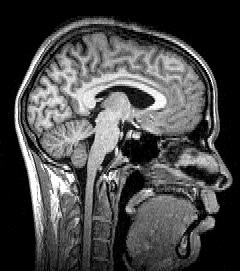
\includegraphics[height=\imageheight]{./images/Sagittal_brain_MRI}%
				\source{w.wiki/7g4}{\ccbysa}%
			}%
			\only<3|handout:2>{%
				\begin{tikzpicture}[remember picture,overlay]%
					\node at (current page.center){%	
						\mode<beamer>{\animategraphics[loop,autoplay,width=\paperwidth,every=\everyframe]{24}{./movies/mouse_skull/mouse_skull}{000}{236}}%
						\mode<handout>{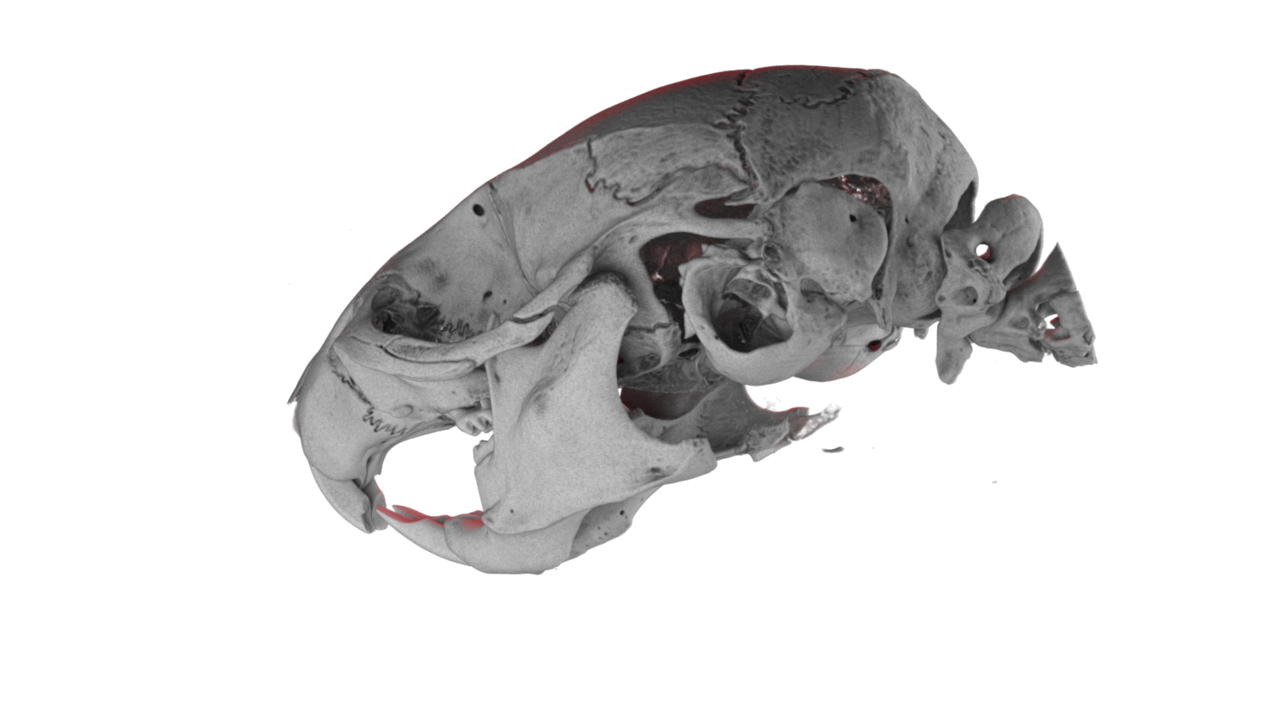
\includegraphics[width=\paperwidth]{./movies/mouse_skull/mouse_skull075}}
					};%
				\end{tikzpicture}%
			}%
		\end{column}%
	\end{columns}%
\end{frame}

\section{(Mikro-)Tomographie}
\begin{frame}
	\frametitle{Computertomographie}
	\centering
	\mode<beamer>{%
		\animategraphics[loop,height=\imageheight,every=\everyframe]{24}{./movies/ct-scanner/ct-scanner0}{001}{480}%
		\source{youtu.be/2CWpZKuy-NE}{}%
		}
	\mode<handout>{%
		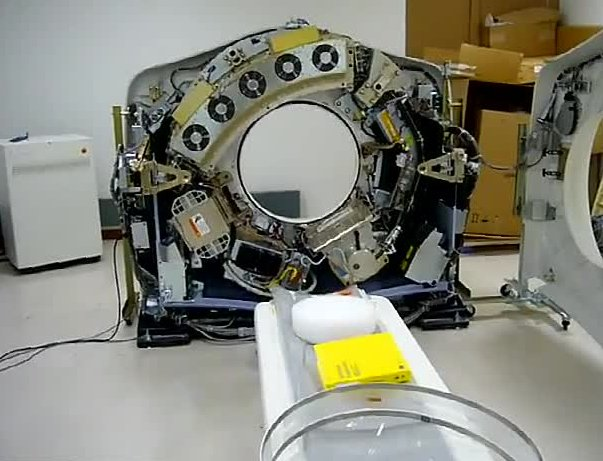
\includegraphics[height=\imageheight]{./movies/ct-scanner/ct-scanner0001}%
		\source{youtu.be/2CWpZKuy-NE}{}%
		}
\end{frame}

\begin{frame}
	\frametitle{\uct}
	\begin{columns}
		\begin{column}{0.49\linewidth}
			\centering
			\documentclass{standalone}
% Draw the setup where the source and detector move, e.g. classic CT
% With help from https://tex.stackexchange.com/q/515519/828
\usepackage{animate}
\usepackage{tikz}
%	\usetikzlibrary{external}
%	\tikzexternalize
%	\tikzsetnextfilename{classicCT}
\usepackage{fontawesome5}	
\usepackage{ifthen}
\ifthenelse{\isundefined{\everyframe}}{%
	% If we're compiling this file via \input, then these variables are already defined.
	% In the other case, we need to define them
	\newcommand{\everyframe}{5}
	\definecolor{ubRed}{HTML}{E6002E}
	% split complementary images from https://www.sessions.edu/color-calculator/
	\definecolor{ubRedComplementary1}{HTML}{00a1e6}
	\definecolor{ubRedComplementary2}{HTML}{00e645}
	\definecolor{ubGrey}{RGB}{217,217,217}
	}{}
\begin{document}
\begin{animateinline}[every=\everyframe]{25}
	\multiframe{180}{n=1+2}{%
%	\tikzifexternalizing{Work-around to make animate happy	}{}%https://tex.stackexchange.com/a/39026/828
		\begin{tikzpicture}
			\pgfdeclarelayer{background}
			\pgfsetlayers{background,main}
			%Help lines
			\draw[<->] (-2.25,0) -- (2.25,0);
			\draw[<->] (0,-2.25) -- (0,2.25);
			\draw[help lines,step=1cm,ultra thin] (-2.45,-2.45) grid (2.45,2.45);
			% Stuff that stays put
			\node[ubRedComplementary1] at (0,0) (sample) {\Huge\faUser};
			% Stuff that moves
			\mode<beamer>{%
				\begin{scope}[rotate around={\n:(sample)}]
				}
				% Rotation arc
				\draw[->, thick,line cap=rect] (1.5,0) arc [start angle=0, end angle=180, radius=1.5];
				\draw[->, thick,line cap=rect] (-1.5,0) arc [start angle=-180, end angle=0, radius=1.5];
				% Source
				\fill[ubRed] (-0.25,1.5) rectangle node (source) [black] {X-ray} +(0.5,0.5);
				% Detector and detector edges
				\fill[ubRedComplementary2,fill] (-0.5,-1.75) rectangle node (detector) [black] {Detektor} +(1,0.25);
				\coordinate (dl) at (-0.45,-1.75);
				\coordinate (dr) at (0.45,-1.75);
				% X-ray cone
				\begin{pgfonlayer}{background}
					\fill[gray,semitransparent] (source.center) -- (dl) -- (dr) -- cycle;
				\end{pgfonlayer}
			\mode<beamer>{%
				\end{scope}
			}
		\end{tikzpicture}
	}
\end{animateinline}
\end{document}

		\end{column}
		\begin{column}{0.49\linewidth}
			\centering
			\only<1>{\documentclass{standalone}
% Draw the setup where the only the sample moves, e.g. microCT
% Essentially just a copy of classicCT in the same folder
\usepackage{animate}
\usepackage{tikz}
%	\usetikzlibrary{external}
%	\tikzexternalize
%	\tikzsetnextfilename{microCT}
\usepackage{fontawesome5}	
\usepackage{ifthen}
\ifthenelse{\isundefined{\everyframe}}{%
	% If we're compiling this file via \input, then these variables are already defined.
	% In the other case, we need to define them
	\newcommand{\everyframe}{5}
	\definecolor{ubRed}{HTML}{E6002E}
	% split complementary images from https://www.sessions.edu/color-calculator/
	\definecolor{ubRedComplementary1}{HTML}{00a1e6}
	\definecolor{ubRedComplementary2}{HTML}{00e645}
	\definecolor{ubGrey}{RGB}{217,217,217}
	}{}
\begin{document}
\begin{animateinline}[every=\everyframe]{25}
	\multiframe{180}{n=1+2}{%
%	\tikzifexternalizing{Work-around to make animate happy	}{}%https://tex.stackexchange.com/a/39026/828
		\begin{tikzpicture}
			\pgfdeclarelayer{background}
			\pgfsetlayers{background,main}
			%Help lines
			\draw[<->] (-2.25,0) -- (2.25,0);
			\draw[<->] (0,-2.25) -- (0,2.25);
			\draw[help lines,step=1cm,ultra thin] (-2.45,-2.45) grid (2.45,2.45);
			% Stuff that stays put
			% Source
			\fill[ubRed] (-0.25,1) rectangle node (source) [black,opacity=0, text opacity=1] {Röntgenquelle} +(0.5,0.5);
			% Detector and detector edges
			\fill[ubRedComplementary2,fill] (-0.5,-1.25) rectangle node (detector) [black] {Detektor} +(1,0.25);
			\coordinate (dl) at (-0.45,-1);
			\coordinate (dr) at (0.45,-1);
			% X-ray cone
			\begin{pgfonlayer}{background}
				\fill[gray,semitransparent] (source.center) -- (dl) -- (dr) -- cycle;
			\end{pgfonlayer}
			% Stuff that moves
			\mode<beamer>{%
				\begin{scope}[rotate around={\n:(0,0)}]
				}
				% Rotation arc
				\draw[->, thick,line cap=rect] (0.618,0) arc [start angle=0, end angle=180, radius=0.618];
				\draw[->, thick,line cap=rect] (-0.618,0) arc [start angle=-180, end angle=0, radius=0.618];
				% Sample
				\node[ubRedComplementary1] at (0,0) (sample) {\rotatebox{\n}{\normalsize\faFish}};
			\mode<beamer>{%
				\end{scope}
				}
		\end{tikzpicture}
	}
\end{animateinline}
\end{document}
}%
			\only<2|handout:0>{\documentclass{standalone}
% Draw the setup where the only the sample moves, e.g. microCT
% Essentially just a copy of classicCT in the same folder
\usepackage{animate}
\usepackage{tikz}
%	\usetikzlibrary{external}
%	\tikzexternalize
%	\tikzsetnextfilename{microCT}
\usepackage{fontawesome5}	
\usepackage{ifthen}
\ifthenelse{\isundefined{\everyframe}}{%
	% If we're compiling this file via \input, then these variables are already defined.
	% In the other case, we need to define them
	\newcommand{\everyframe}{5}
	\definecolor{ubRed}{HTML}{E6002E}
	% split complementary images from https://www.sessions.edu/color-calculator/
	\definecolor{ubRedComplementary1}{HTML}{00a1e6}
	\definecolor{ubRedComplementary2}{HTML}{00e645}
	\definecolor{ubGrey}{RGB}{217,217,217}
	}{}
\begin{document}
\begin{animateinline}[every=\everyframe]{25}
	\multiframe{180}{n=1+2}{%
%	\tikzifexternalizing{Work-around to make animate happy	}{}%https://tex.stackexchange.com/a/39026/828
		\begin{tikzpicture}
			\pgfdeclarelayer{background}
			\pgfsetlayers{background,main}
			%Help lines
			\draw[<->] (-2.25,0) -- (2.25,0);
			\draw[<->] (0,-2.25) -- (0,2.25);
			\draw[help lines,step=1cm,ultra thin] (-2.45,-2.45) grid (2.45,2.45);
			% Stuff that stays put
			% Source
			\fill[ubRed] (-0.25,1) rectangle node (source) [black,opacity=0, text opacity=1] {X-ray} +(0.5,0.5);
			% Detector and detector edges
			\fill[ubRedComplementary2,fill] (-0.5,-1.25) rectangle node (detector) [black] {Detektor} +(1,0.25);
			\coordinate (dl) at (-0.45,-1);
			\coordinate (dr) at (0.45,-1);
			% X-ray cone
			\begin{pgfonlayer}{background}
				\fill[gray,semitransparent] (source.center) -- (dl) -- (dr) -- cycle;
			\end{pgfonlayer}
			% Stuff that moves
			\mode<beamer>{%
				\begin{scope}[rotate around={\n:(0,-0.5)}]
				}
				% Rotation arc
				\draw[->, thick,line cap=rect] (0.618,-0.5) arc [start angle=0, end angle=180, radius=0.618];
				\draw[->, thick,line cap=rect] (-0.618,-0.5) arc [start angle=-180, end angle=0, radius=0.618];
				% Sample
				\node[ubRedComplementary1] at (0,-0.5) (sample) {\rotatebox{\n}{\huge\faFish}};
			\mode<beamer>{%
				\end{scope}
				}
		\end{tikzpicture}
	}
\end{animateinline}
\end{document}
}%
			\only<3|handout:0>{\documentclass{standalone}
% Draw the setup where the only the sample moves, e.g. microCT
% Essentially just a copy of classicCT in the same folder
\usepackage{animate}
\usepackage{tikz}
%	\usetikzlibrary{external}
%	\tikzexternalize
%	\tikzsetnextfilename{microCT}
\usepackage{fontawesome5}	
\usepackage{ifthen}
\ifthenelse{\isundefined{\everyframe}}{%
	% If we're compiling this file via \input, then these variables are already defined.
	% In the other case, we need to define them
	\newcommand{\everyframe}{5}
	\definecolor{ubRed}{HTML}{E6002E}
	% split complementary images from https://www.sessions.edu/color-calculator/
	\definecolor{ubRedComplementary1}{HTML}{00a1e6}
	\definecolor{ubRedComplementary2}{HTML}{00e645}
	\definecolor{ubGrey}{RGB}{217,217,217}
	}{}
\begin{document}
\begin{animateinline}[every=\everyframe]{25}
	\multiframe{180}{n=1+2}{%
%	\tikzifexternalizing{Work-around to make animate happy	}{}%https://tex.stackexchange.com/a/39026/828
		\begin{tikzpicture}
			\pgfdeclarelayer{background}
			\pgfsetlayers{background,main}
			%Help lines
			\draw[<->] (-2.25,0) -- (2.25,0);
			\draw[<->] (0,-2.25) -- (0,2.25);
			\draw[help lines,step=1cm,ultra thin] (-2.45,-2.45) grid (2.45,2.45);
			% Stuff that stays put
			% Source
			\fill[ubRed] (-0.25,1) rectangle node (source) [black,opacity=0, text opacity=1] {Röntgenquelle} +(0.5,0.5);
			% Detector and detector edges
			\fill[ubRedComplementary2,fill] (-0.5,-1.25) rectangle node (detector) [black] {Detektor} +(1,0.25);
			\coordinate (dl) at (-0.45,-1);
			\coordinate (dr) at (0.45,-1);
			% X-ray cone
			\begin{pgfonlayer}{background}
				\fill[gray,semitransparent] (source.center) -- (dl) -- (dr) -- cycle;
			\end{pgfonlayer}
			% Stuff that moves
			\mode<beamer>{%
				\begin{scope}[rotate around={\n:(0,0.5)}]
				}
				% Rotation arc
				\draw[->, thick,line cap=rect] (0.618,0.5) arc [start angle=0, end angle=180, radius=0.618];
				\draw[->, thick,line cap=rect] (-0.618,0.5) arc [start angle=-180, end angle=0, radius=0.618];
				% Sample
				\node[ubRedComplementary1] at (0,0.5) (sample) {\rotatebox{\n}{\tiny\faFish}};
			\mode<beamer>{%
				\end{scope}
				}
		\end{tikzpicture}
	}
\end{animateinline}
\end{document}
}%
		\end{column}
	\end{columns}
\end{frame}

\begin{frame}
	\frametitle{Why \uct?}
	\begin{columns}
		\begin{column}{0.49\linewidth}
			% https://www.cancerimagingarchive.net/nbia-search/?saved-cart=nbia-76761575299081509
			\only<1-4|handout:1-4>{%
				\pgfmathsetlength{\imagewidth}{\imagewidth}%
				\pgfmathsetlength{\imagescale}{\imagewidth/512}%
				\def\x{316}% scalebar-x starting at golden ratio of image width of 512px = 316
				\def\y{361}% scalebar-y at 90% of image height of 401px = 361
				\begin{tikzpicture}[x=\imagescale,y=-\imagescale]
					\node[anchor=north west, inner sep=0pt, outer sep=0pt] at (0,0) {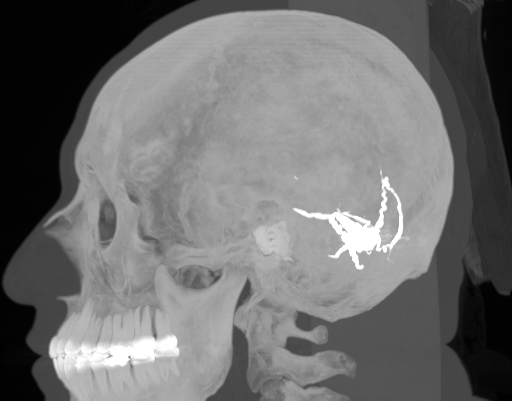
\includegraphics[width=\imagewidth]{./images/comparison/MAX_human}};
					% 512.000px = 250.0096mm -> 100px = 48830.000um -> 1.024px = 500um, 0.205px = 100um
					%\draw[|-|,blue,thick] (0,200) -- (512,200) node [sloped,midway,above,fill=white,semitransparent,text opacity=1] {\SI{250.0096}{\milli\meter} (512px) TEMPORARY!};
					\draw[|-|,white,shadowed] (\x,\y) -- (\x+102.4,\y) node [midway,above] {\shadowtext{\SI{5}{\centi\meter}}};
				\end{tikzpicture}%
			}%
			\only<5|handout:0>{%
				\pgfmathsetlength{\imagewidth}{\imagewidth}%
				\pgfmathsetlength{\imagescale}{\imagewidth/512}%
				\def\x{316}% scalebar-x starting at golden ratio of image width of 512px = 316
				\def\y{361}% scalebar-y at 90% of image height of 401px = 361
				\def\mag{6}% magnification of inset
				\def\size{125}% size of inset
				\begin{tikzpicture}[x=\imagescale,y=-\imagescale,spy using outlines={rectangle,magnification=\mag,size=\size,connect spies}]
					\node[anchor=north west, inner sep=0pt, outer sep=0pt] at (0,0) {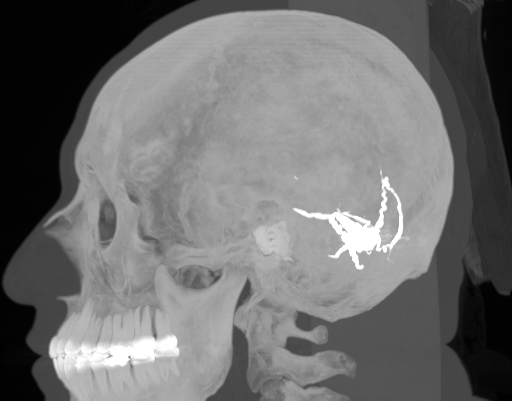
\includegraphics[width=\imagewidth]{./images/comparison/MAX_human}};
					\spy [ubRed] on (58,356) in node at (256,201) [anchor=center];
					% 512.000px = 250.0096mm -> 100px = 48830.000um -> 1.024px = 500um, 0.205px = 100um
					\draw[|-|,white,shadowed] (\x,\y) -- (\x+102.4,\y) node [midway,above] {\shadowtext{\SI{5}{\centi\meter}}};
				\end{tikzpicture}%
			}%
			\renewcommand{\imagewidth}{0.1554\columnwidth}%
			\only<6|handout:5>{%
				\centering
				\pgfmathsetlength{\imagewidth}{\imagewidth}%
				\pgfmathsetlength{\imagescale}{\imagewidth/512}%
				\def\x{316}% scalebar-x starting at golden ratio of image width of 512px = 316
				\def\y{361}% scalebar-y at 90% of image height of 401px = 361
				\begin{tikzpicture}[x=\imagescale,y=-\imagescale]
					\node[anchor=north west, inner sep=0pt, outer sep=0pt] at (0,0) {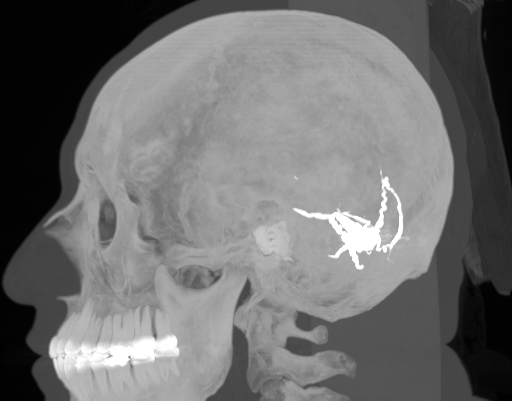
\includegraphics[width=\imagewidth]{./images/comparison/MAX_human}};
					% 512.000px = 250.0096mm -> 100px = 48830.000um -> 1.024px = 500um, 0.205px = 100um
					\draw[|-|,white,shadowed] (\x,\y) -- (\x+102.4,\y) node [midway,above] {\shadowtext{\SI{5}{\centi\meter}}};
				\end{tikzpicture}%
			}%
			\sourcecite{Clark2013}{Subject \emph{C3L-02465}}
		\end{column}%
		\begin{column}{0.49\linewidth}
			\only<1|handout:1>{%
				\pgfmathsetlength{\imagewidth}{\imagewidth}%
				\pgfmathsetlength{\imagescale}{\imagewidth/3295}%
				\def\x{2036}% scalebar-x starting at golden ratio of image width of 3295px = 2036
				\def\y{1343}% scalebar-y at 90% of image height of 1492px = 1343
				\begin{tikzpicture}[x=\imagescale,y=-\imagescale]
					\node[anchor=north west, inner sep=0pt, outer sep=0pt] at (0,0) {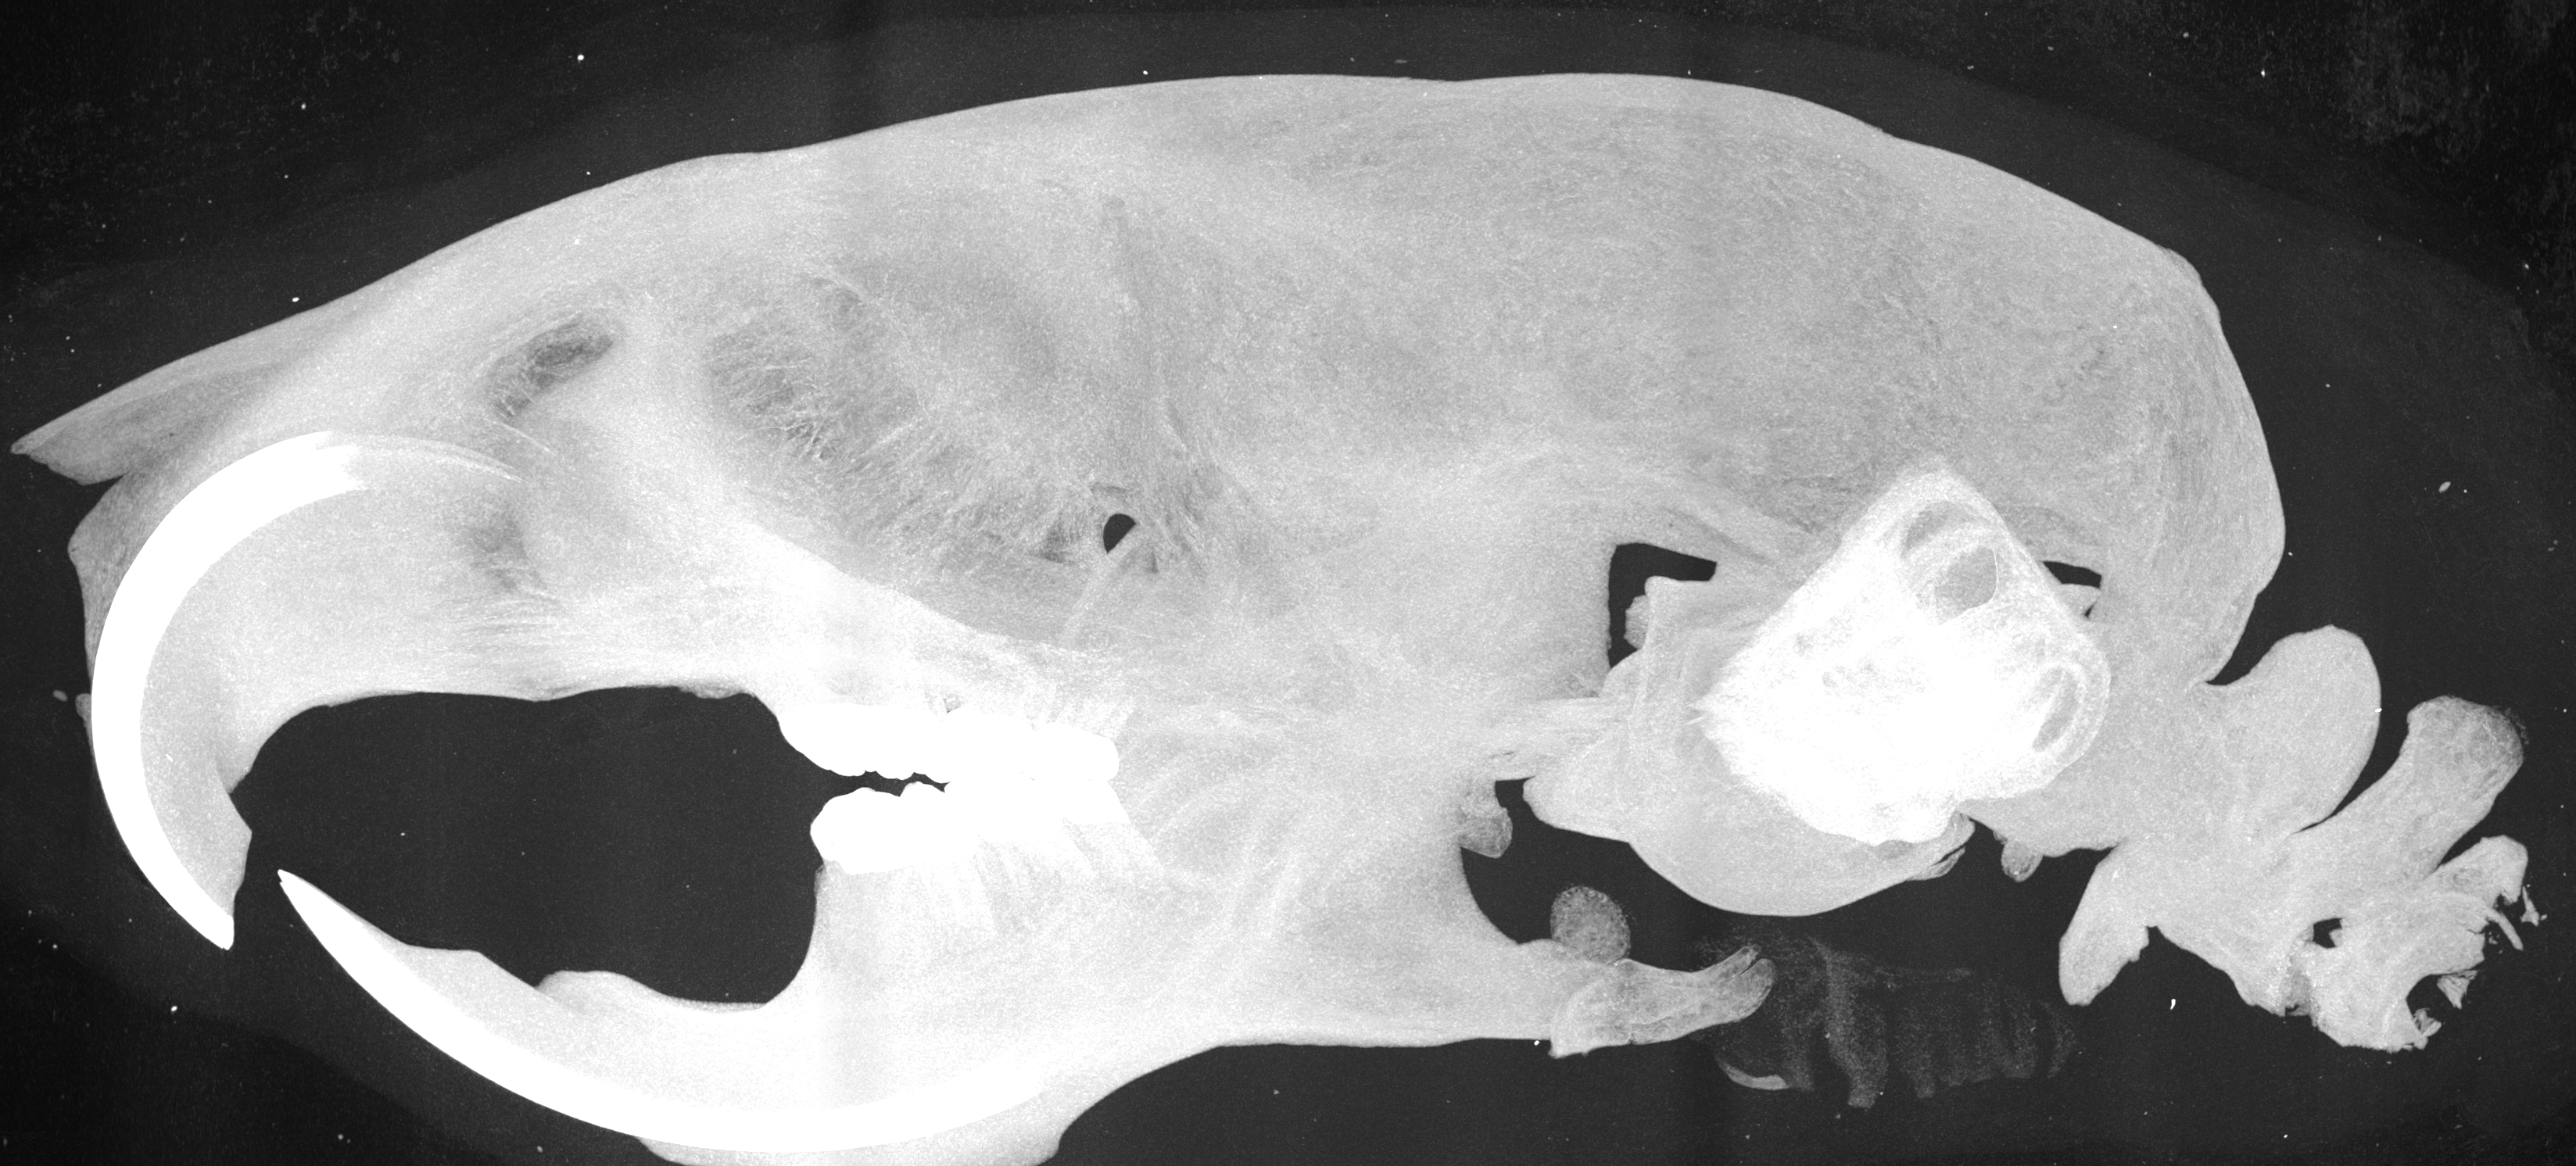
\includegraphics[width=\imagewidth]{./images/comparison/MAX_mouse}};
					% 3295.000px = 26.2282mm -> 100px = 796.000um -> 62.814px = 500um, 12.563px = 100um
					%\draw[|-|,blue,thick] (0,746) -- (3295,746) node [sloped,midway,above,fill=white,semitransparent,text opacity=1] {\SI{26.2282}{\milli\meter} (3295px) TEMPORARY!};
					\draw[|-|,white,shadowed] (\x,\y) -- (\x+628.14,\y) node [midway,above] {\shadowtext{\SI{5}{\milli\meter}}};
				\end{tikzpicture}%
			}%
			\renewcommand{\imagewidth}{0.1\columnwidth}%
			\only<2|handout:2>{%
				\centering
				\pgfmathsetlength{\imagewidth}{\imagewidth}%
				\pgfmathsetlength{\imagescale}{\imagewidth/54}%
				\def\x{33}% scalebar-x starting at golden ratio of image width of 54px = 33
				\def\y{22}% scalebar-y at 90% of image height of 24px = 22
				\begin{tikzpicture}[x=\imagescale,y=-\imagescale]
					\node[anchor=north west, inner sep=0pt, outer sep=0pt] at (0,0) {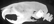
\includegraphics[width=\imagewidth]{./images/comparison/MAX_mouse_488umppx}};
					% 54.000px = 26.3682mm -> 100px = 48830.000um -> 1.024px = 500um, 0.205px = 100um
					%\draw[|-|,blue,thick] (0,12) -- (54,12) node [sloped,midway,above,fill=white,semitransparent,text opacity=1] {\SI{26.3682}{\milli\meter} (54px) TEMPORARY!};
					\draw[|-|,white,shadowed] (\x,\y) -- (\x+102.4,\y) node [midway,above] {\shadowtext{\SI{5}{\centi\meter}}};
					%\draw[color=red, anchor=south west] (0,24) node [fill=white, semitransparent] {Legend} node {Legend};
				\end{tikzpicture}%
			}%
			\renewcommand{\imagewidth}{\columnwidth}
			\only<3|handout:3>{%
				\centering
				\pgfmathsetlength{\imagewidth}{\imagewidth}%
				\pgfmathsetlength{\imagescale}{\imagewidth/54}%
				\def\x{33}% scalebar-x starting at golden ratio of image width of 54px = 33
				\def\y{22}% scalebar-y at 90% of image height of 24px = 22
				\begin{tikzpicture}[x=\imagescale,y=-\imagescale]
					\node[anchor=north west, inner sep=0pt, outer sep=0pt] at (0,0) {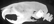
\includegraphics[width=\imagewidth]{./images/comparison/MAX_mouse_488umppx}};
					% 54.000px = 26.3682mm -> 100px = 48830.000um -> 1.024px = 500um, 0.205px = 100um
					%\draw[|-|,blue,thick] (0,12) -- (54,12) node [sloped,midway,above,fill=white,semitransparent,text opacity=1] {\SI{26.3682}{\milli\meter} (54px) TEMPORARY!};
					\draw[|-|,white,shadowed] (\x,\y) -- (\x+10.24,\y) node [midway,above] {\shadowtext{\SI{5}{\milli\meter}}};
					%\draw[color=red, anchor=south west] (0,24) node [fill=white, semitransparent] {Legend} node {Legend};
				\end{tikzpicture}%
			}%
			\only<4|handout:4>{%
				\pgfmathsetlength{\imagewidth}{\imagewidth}%
				\pgfmathsetlength{\imagescale}{\imagewidth/3295}%
				\def\x{2036}% scalebar-x starting at golden ratio of image width of 3295px = 2036
				\def\y{1343}% scalebar-y at 90% of image height of 1492px = 1343
				\begin{tikzpicture}[x=\imagescale,y=-\imagescale]
					\node[anchor=north west, inner sep=0pt, outer sep=0pt] at (0,0) {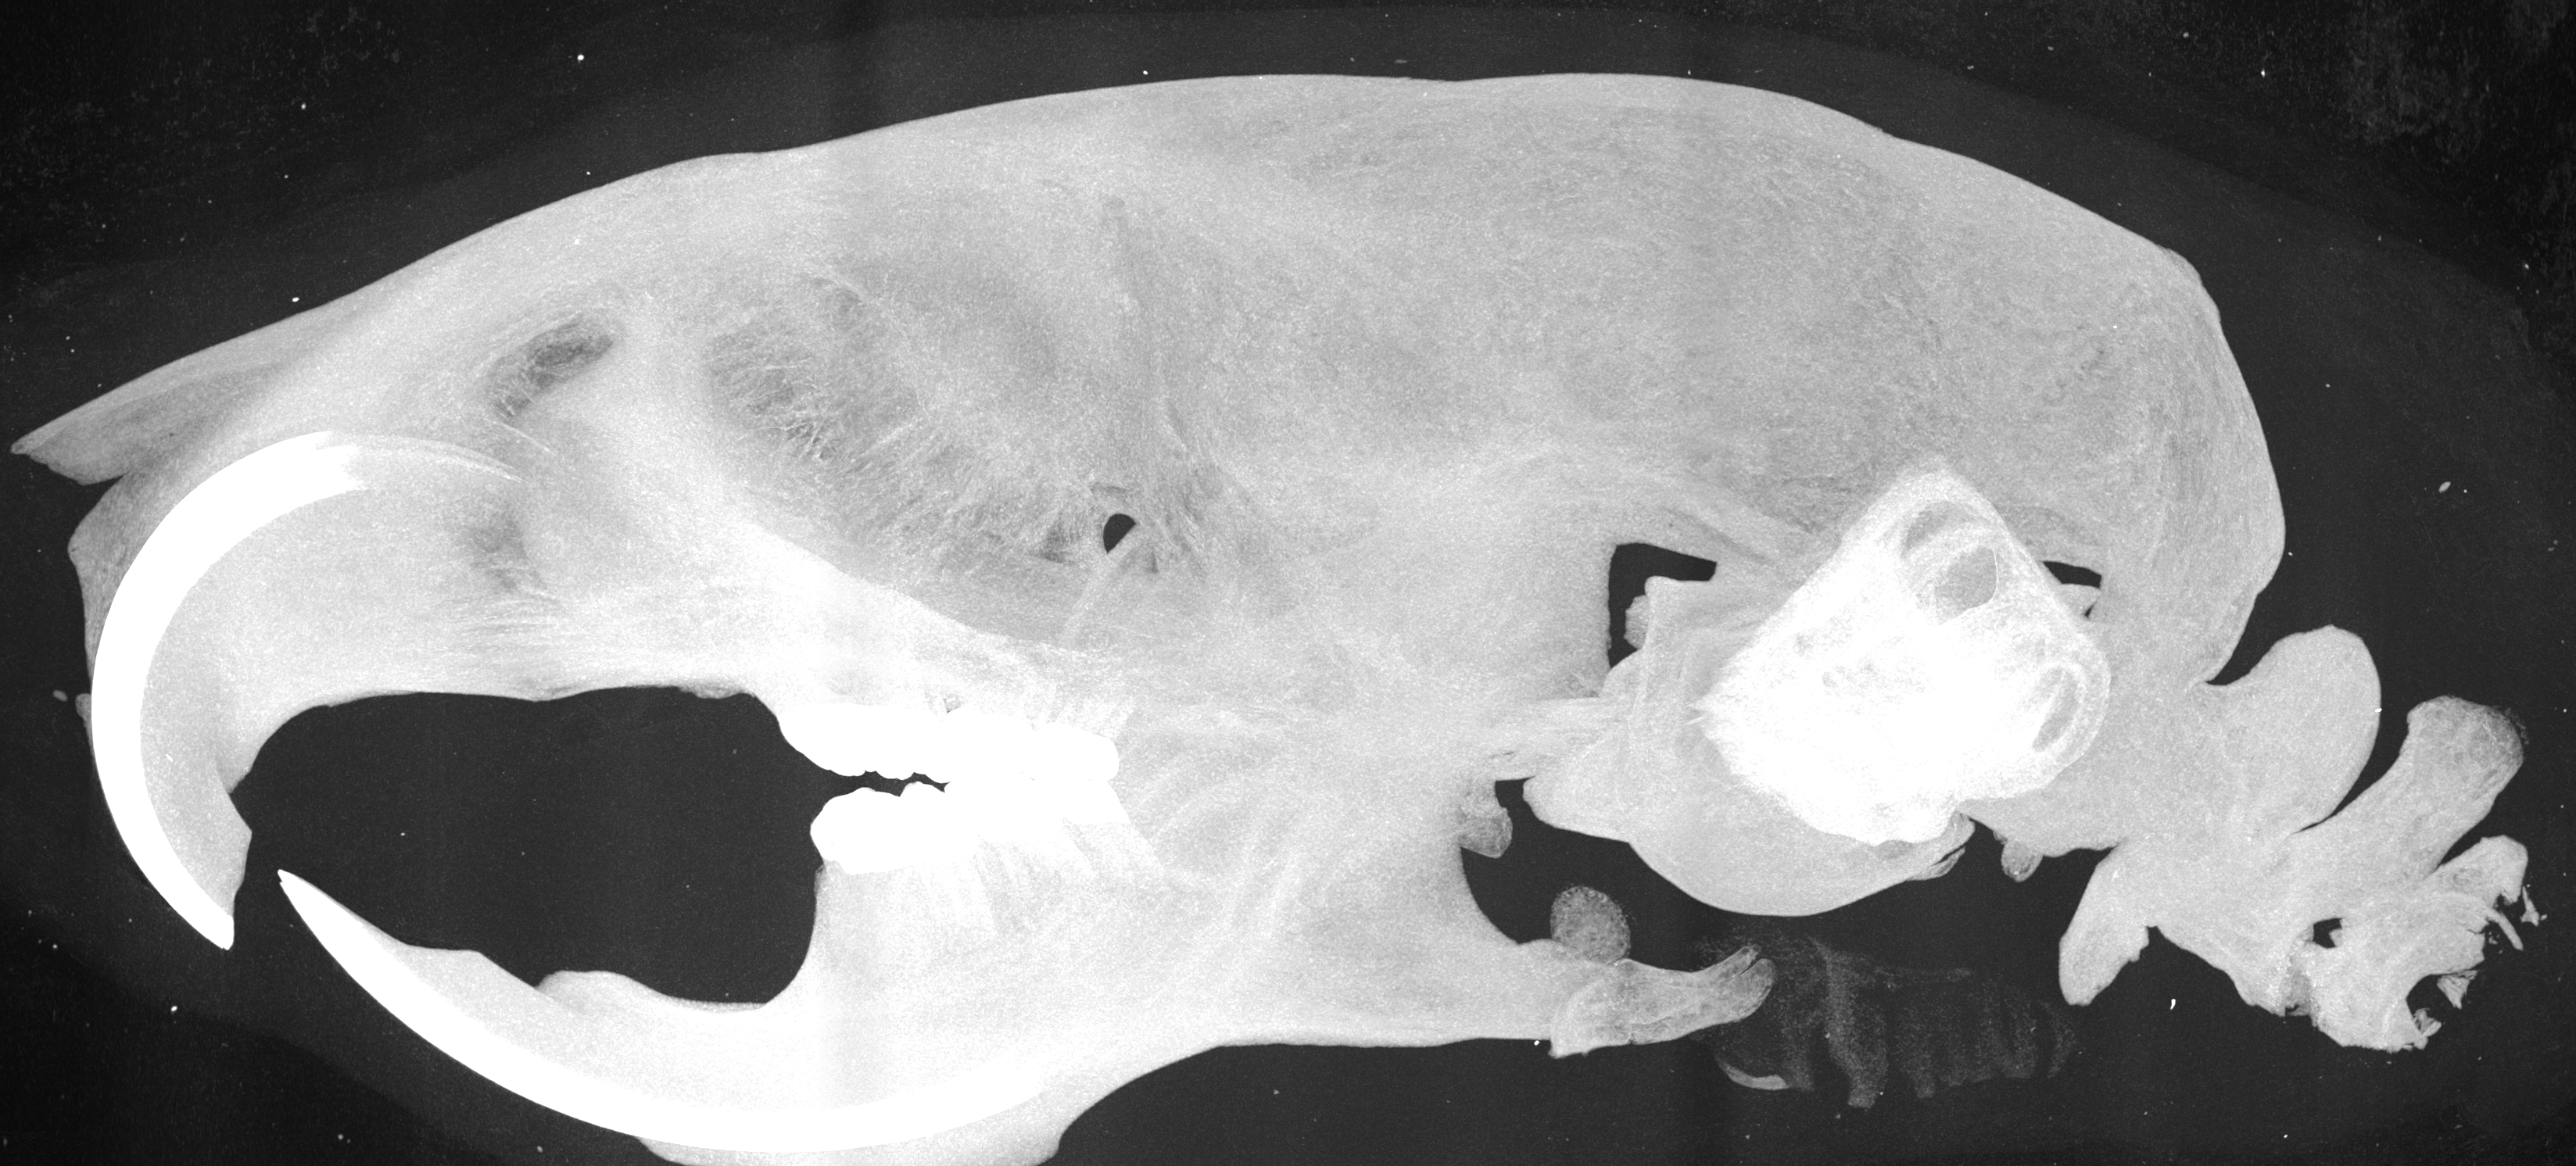
\includegraphics[width=\imagewidth]{./images/comparison/MAX_mouse}};
					% 3295.000px = 26.2282mm -> 100px = 796.000um -> 62.814px = 500um, 12.563px = 100um
					\draw[|-|,white,shadowed] (\x,\y) -- (\x+628.14,\y) node [midway,above] {\shadowtext{\SI{5}{\milli\meter}}};
				\end{tikzpicture}%
			}%
			\only<5|handout:0>{%
				\pgfmathsetlength{\imagewidth}{\imagewidth}%
				\pgfmathsetlength{\imagescale}{\imagewidth/3295}%
				\def\x{2036}% scalebar-x starting at golden ratio of image width of 3295px = 2036
				\def\y{1343}% scalebar-y at 90% of image height of 1492px = 1343
				\def\mag{6}% magnification of inset
				\def\size{125}% size of inset
				\begin{tikzpicture}[x=\imagescale,y=-\imagescale,spy using outlines={rectangle,magnification=\mag,size=\size,connect spies}]
					\node[anchor=north west, inner sep=0pt, outer sep=0pt] at (0,0) {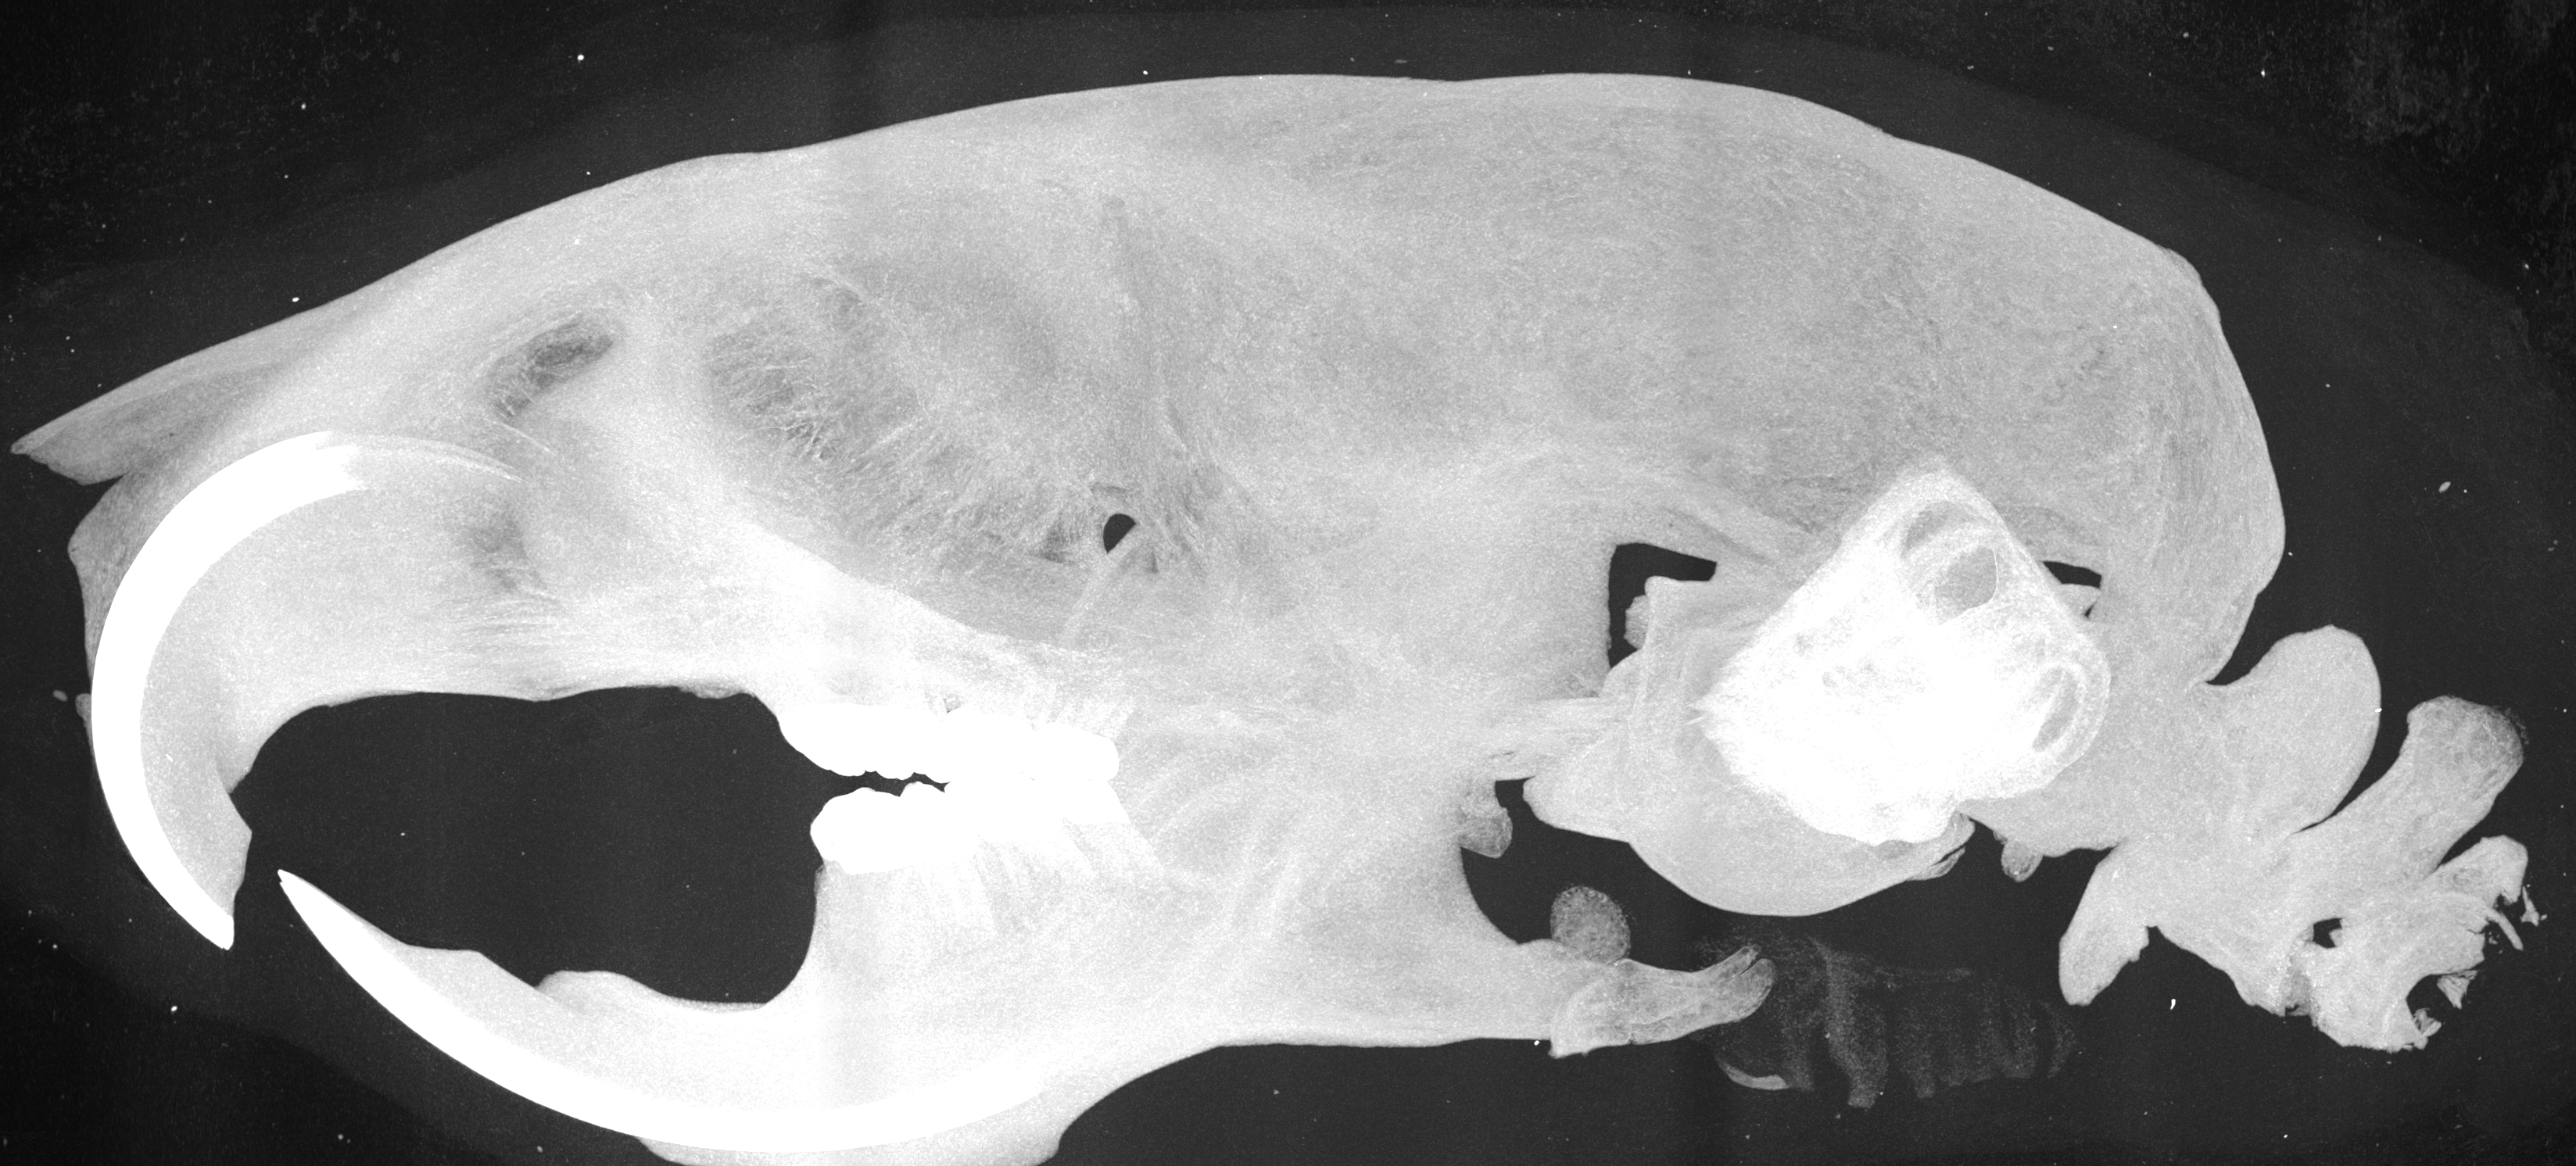
\includegraphics[width=\imagewidth]{./images/comparison/MAX_mouse}};
					\spy [ubRed] on (352,1116) in node at (1648,746) [anchor=center];
					% 3295.000px = 26.2282mm -> 100px = 796.000um -> 62.814px = 500um, 12.563px = 100um
					\draw[|-|,white,shadowed] (\x,\y) -- (\x+628.14,\y) node [midway,above] {\shadowtext{\SI{5}{\milli\meter}}};
				\end{tikzpicture}%
			}%
			\only<6|handout:5>{%
				\pgfmathsetlength{\imagewidth}{\imagewidth}%
				\pgfmathsetlength{\imagescale}{\imagewidth/3295}%
				\def\x{2036}% scalebar-x starting at golden ratio of image width of 3295px = 2036
				\def\y{1343}% scalebar-y at 90% of image height of 1492px = 1343
				\begin{tikzpicture}[x=\imagescale,y=-\imagescale]
					\node[anchor=north west, inner sep=0pt, outer sep=0pt] at (0,0) {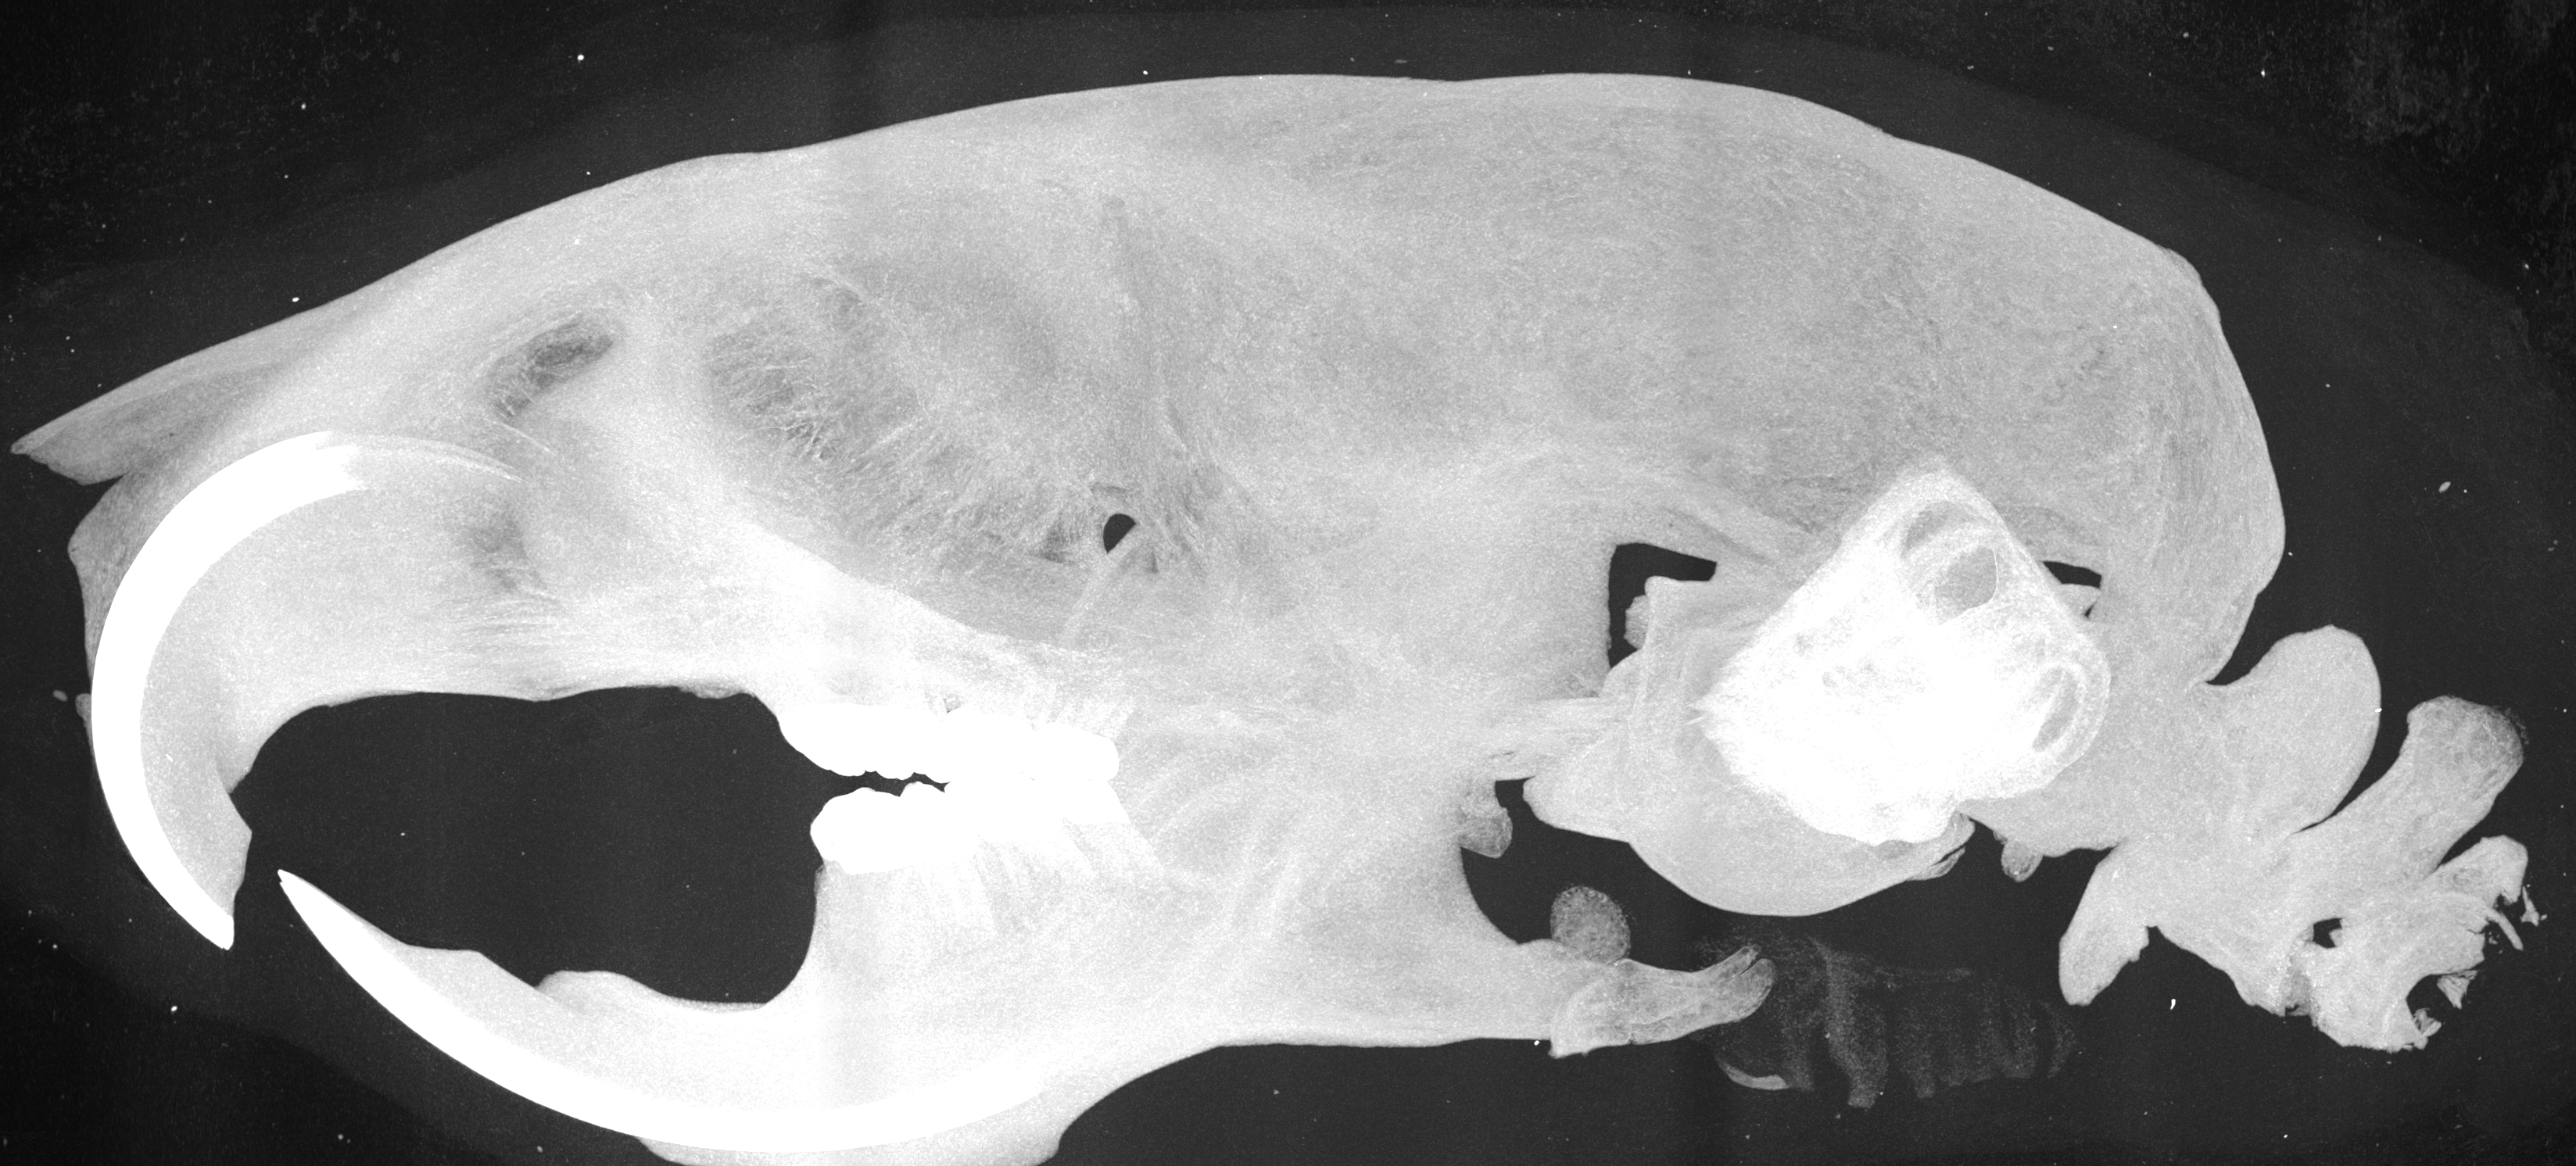
\includegraphics[width=\imagewidth]{./images/comparison/MAX_mouse}};
					% 3295.000px = 26.2282mm -> 100px = 796.000um -> 62.814px = 500um, 12.563px = 100um
					\draw[|-|,white,shadowed] (\x,\y) -- (\x+628.14,\y) node [midway,above] {\shadowtext{\SI{5}{\milli\meter}}};
				\end{tikzpicture}%
			}%
		\end{column}
	\end{columns}
\end{frame}
\note{The human head scan was downloaded from the \href{https://www.cancerimagingarchive.net}{Cancer Imaging Archive}.
	We loaded the DICOM slices in Fiji, resliced it to show it from the side and then used to generate an MIP.
	According to the DICOM tags, the voxel size is \qtyproduct{0.4883 x 0.4883 x 0.625}{\milli\meter}, the image size is 512\(\times\)512 pixels.
	The mouse head is the same as shown in the early animation.
	The files from the early animation were resized 0.25 times; here we used the original dataset (Mouse1265\_Skull\_Gaby\_TKI\_7\_96um\_Al05\_2K) for a reslice and the generation of the MIP.
	The voxel size of the original data is 7.96 um, the image size is 3295\(\times\)1492 pixels.
}

\begin{frame}
	\frametitle{\uct in der Histologie}
	\begin{itemize}
		\item Zerstörungsfrei
		\item Virtuelle Schnitte in \emph{jeder} Richtung
		\item \emph{Richtige} Histologie ist danach immer noch möglich
	\end{itemize}
\end{frame}

% The TOMCAT data is at \\resstore.unibe.ch\ana_rs_schittny\data\Gruppe\AnaTera\AnaTera4\share\SLS\2010a\mrg\
\begin{frame}[label=current]
	\frametitle{\uct in der Histologie}
	\begin{columns}
		\begin{column}{0.49\linewidth}
			\centering
			\tikzset{shadowed/.style={preaction={transform canvas={shift={(1pt,-1pt)}},draw=green, thick}}} % shadowed drawing https://tex.stackexchange.com/a/185853/828
			\pgfmathsetlength{\imagescale}{\imagewidth/2576}%
			\def\x{1592}% scalebar-x starting at golden ratio of image width of 2576px = 1592
			\def\y{1739}% scalebar-y at 90% of image height of 1932px = 1739
			\def\mag{4}% magnification of inset
			\def\size{75}% size of inset
			\begin{tikzpicture}[x=\imagescale,y=-\imagescale,spy using outlines={rectangle,magnification=\mag,size=\size,connect spies}]
				\node[anchor=north west, inner sep=0pt, outer sep=0pt] at (0,0) {\includegraphics[width=\imagewidth]{./images/R108C04A_II_8_0.tif-corrected.png}};
				\spy [red] on (2276,1632) in node at (0,0) [anchor=north west];
				% 2576.000px = 1.3910400000000003mm -> 100px = 54.000um -> 925.926px = 500um, 185.185px = 100um
				\draw[|-|,white,thick,shadowed] (\x,\y) -- (\x+925.926,\y) node [midway,above] {\shadowtext{\SI{500}{\micro\meter}}};
			\end{tikzpicture}%
		\end{column}
		\begin{column}{0.49\linewidth}
			\centering
			\tikzset{shadowed/.style={preaction={transform canvas={shift={(1pt,-1pt)}},draw=green, thick}}} % shadowed drawing https://tex.stackexchange.com/a/185853/828
			\pgfmathsetlength{\imagescale}{\imagewidth/2936}%
			\def\x{1814}% scalebar-x starting at golden ratio of image width of 2936px = 1814
			\def\y{1030}% scalebar-y at 90% of image height of 1145px = 1030
			\def\mag{4}% magnification of inset
			\def\size{75}% size of inset
			\begin{tikzpicture}[x=\imagescale,y=-\imagescale,spy using outlines={rectangle,magnification=\mag,size=\size,connect spies}]
				\node[anchor=north west, inner sep=0pt, outer sep=0pt] at (0,0) {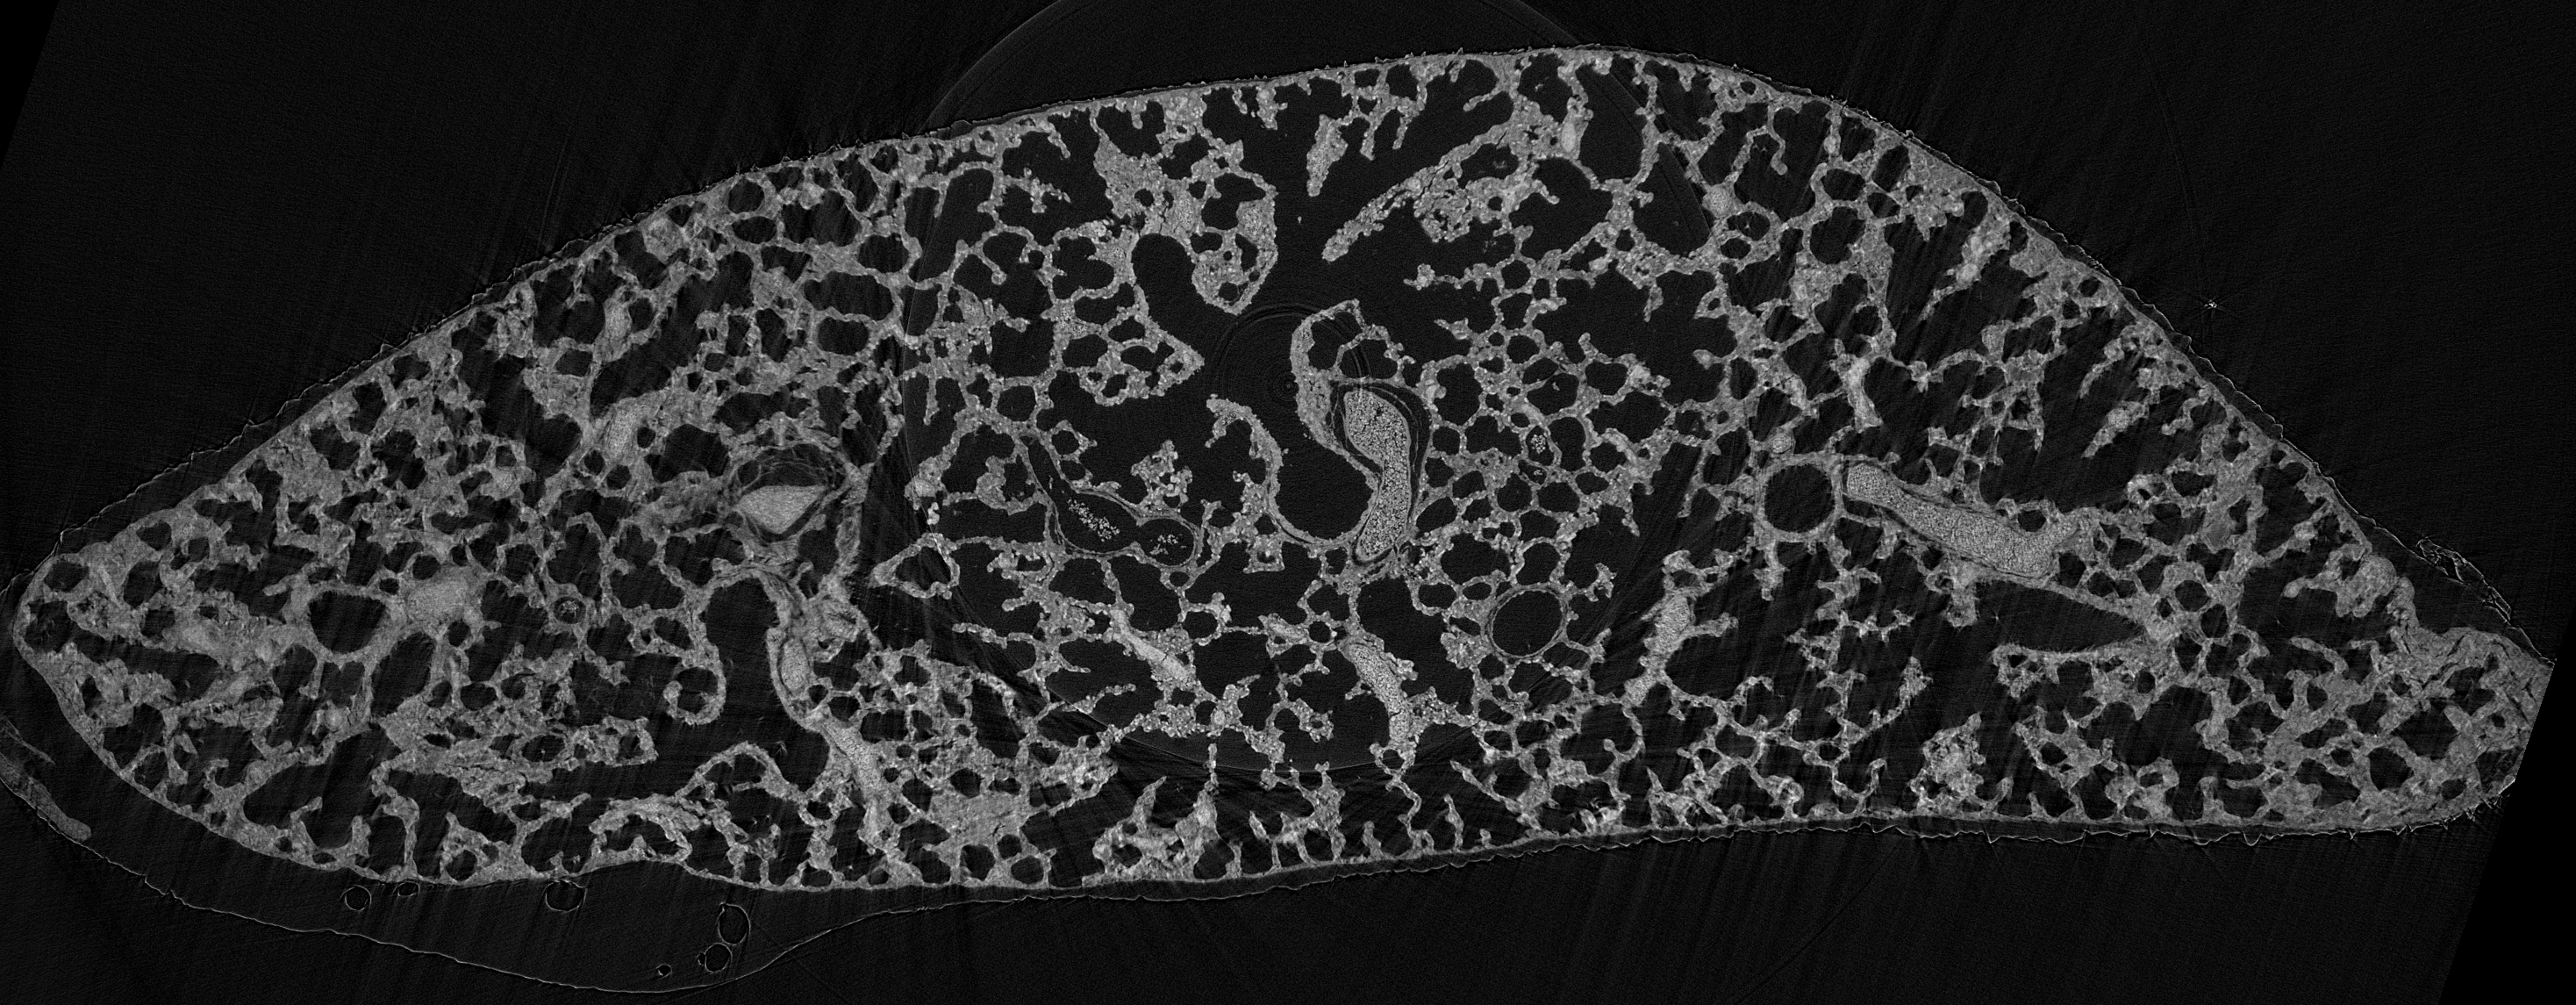
\includegraphics[width=\imagewidth]{./images/R108C04At-mrg1024.rec.8bit.png}};
				\spy [red] on (2636,845) in node at (0,0) [anchor=north west];
				% 2936.000px = 4.34528mm -> 100px = 148.000um -> 337.838px = 500um, 67.568px = 100um
				\draw[|-|,white,thick,shadowed] (\x,\y) -- (\x+337.838,\y) node [midway,above] {\shadowtext{\SI{500}{\micro\meter}}};
			\end{tikzpicture}%
		\end{column}
	\end{columns}
	\centering
	Bilder aus \cite{Haberthuer2021a}
\end{frame}

\begin{frame}
	\frametitle{\uct in der Histologie}
	\begin{itemize}
		\item Virtuelle Schnitte in \emph{jeder} Richtung
		\item Zeigen von solchen virtuellen Schnitten, z.B. anhand des Maus-Scans für Dea
	\end{itemize}
\end{frame}

\renewcommand{\imagewidth}{0.618\linewidth}
\begin{frame}[label=current]
	\frametitle{\uct im Vergleich mit EM}
	\begin{columns}
		\begin{column}{0.49\linewidth}
			\centering
			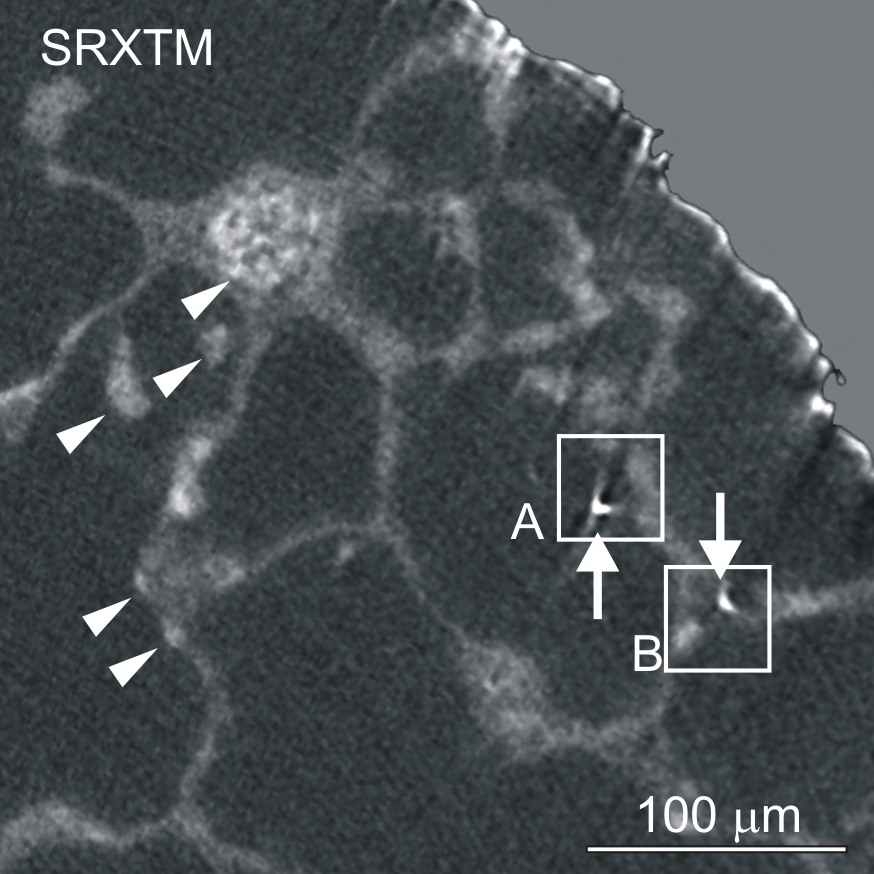
\includegraphics[width=\imagewidth]{./images/gold-nanoparticles-srxtm}
		\end{column}
		\begin{column}{0.49\linewidth}
			\centering
			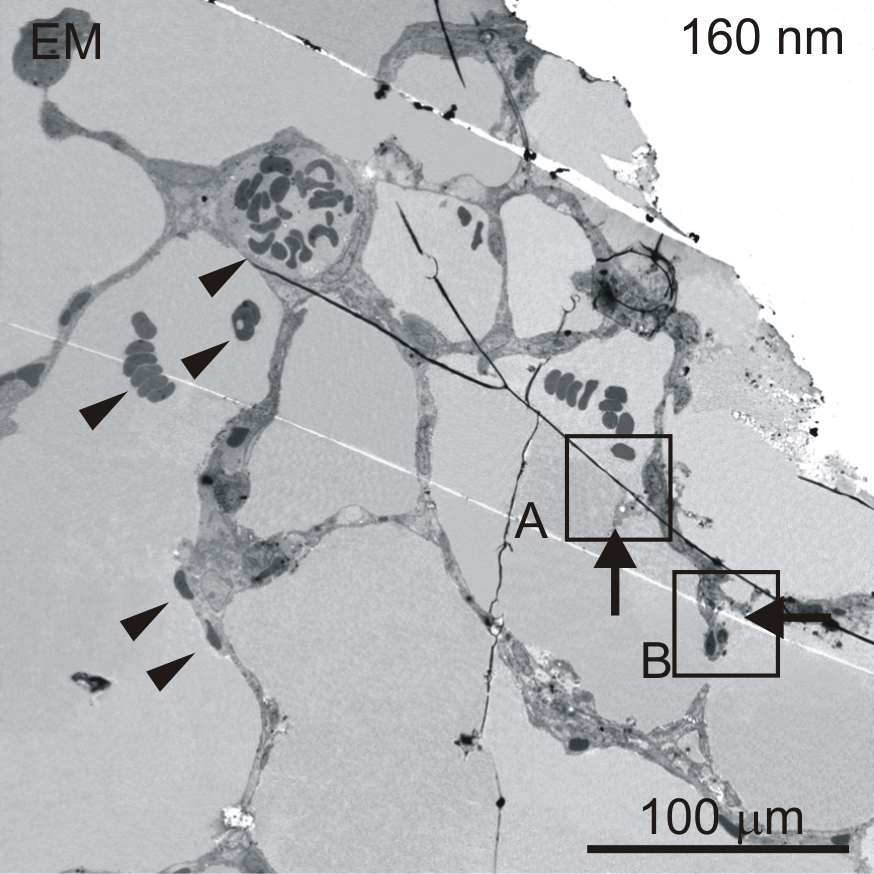
\includegraphics[width=\imagewidth]{./images/gold-nanoparticles-em}			
		\end{column}
	\end{columns}
	\centering
	Bilder aus \cite{Haberthuer2009}
\end{frame}			
		
\begin{frame}
	\frametitle{Adiömersi!}
\end{frame}

\mode<beamer>{\begin{frame}[shrink=20]}
\mode<handout>{\begin{frame}[allowframebreaks]}
	\frametitle{Literatur}
	\mode<beamer>{\renewcommand*{\bibfont}{\tiny}}
	\mode<handout>{\renewcommand*{\bibfont}{\scriptsize}}
	\setbeamertemplate{bibliography item}{\insertbiblabel}
	\printbibliography
\end{frame}

\end{document}
